\documentclass[11pt]{amsart}
\usepackage{geometry}                % See geometry.pdf to learn the layout options. There are lots.
\geometry{letterpaper}                   % ... or a4paper or a5paper or ... 
%\geometry{landscape}                % Activate for for rotated page geometry
\usepackage[parfill]{parskip}    % Activate to begin paragraphs with an empty line rather than an indent
\usepackage{graphicx}
\usepackage{amssymb}
\usepackage{epstopdf}

\DeclareGraphicsRule{.tif}{png}{.png}{`convert #1 `dirname #1`/`basename #1 .tif`.png}
\setcounter{secnumdepth}{5}

\title[Scene Completion and Image Resizing]{Implementing a Scene Completion Algorithm with a Dynamic Image Resizing Extension}
\author{Matthew Conlen \\ Michael Gisi  \\ EECS 442 \\ University of Michigan}
\date{}                                           % Activate to display a given date or no date

\begin{document}
\maketitle

\begin{abstract}
The problem of scene completion has received much attention in recent computer vision research. We 
look at a solution proposed by Hays and Effros \cite{Hays:2007}. We provide our own implementation of the
algorithm proposed in \cite{Hays:2007} and examine the results. We also propose a method of using this 
scene completion algorithm to dynamically resize images using the seam carving algorithm
given by Avidan and Shamir \cite{Avidan:2007}. We consider the benefits and drawbacks that are associated with the previously mentioned methods of scene completion and image resizing. These methods are computationally expensive and rely on a local database of millions of images to achieve satisfactory results. This makes the algorithm intractable for widespread use, but we consider possible remedies for this in our future work section. 
 
\end{abstract}

\section{Introduction}

In this paper we consider an algorithm for scene completion based on work by Hays and Effros \cite{Hays:2007}. This algorithm allows a user to select an area of a picture and then algorithmically fills that area in with different visual content from another image. This is a difficult problem because the content that is added to the image must look as if it was part of the image originally. 

There are many reasons why a person would wish to remove part of an image. For example, perhaps some passers-by have entered into the background and ruined an otherwise beautiful image. It may be the case that a person is in the photograph who has fallen out of favor (e.g. an ex-girlfriend), or maybe there is politically incendiary content that needs to be removed \cite{King:1997}. As further evidence that this problem is relevant outside of the academic world, Adobe Photoshop CS5 (the most recent version of the popular image editing software at time of writing ) features a new tool called ``Content-Aware Fill'' that allows users to remove certain areas from their images \cite{Barnes:2009}. 

The scene completion method presented by Hays and Effros is designed to take advantage of the plethora of data currently available on the internet. The intuition behind the algorithm is to compile a large database of images and then, when it is time to do scene completion, try using a subset of these images that is semantically close to the original. For each image in this subset, its optimal scale and position is calculated and then the relevant area of that image is pasted into the original scene. Some post processing is done to make the entire scene look more natural. This method is displayed graphically in Figure \ref{scene}. As the size of the image database is increased, so will the believability of the scene completion.

\begin{figure}[htbp]
\begin{center}
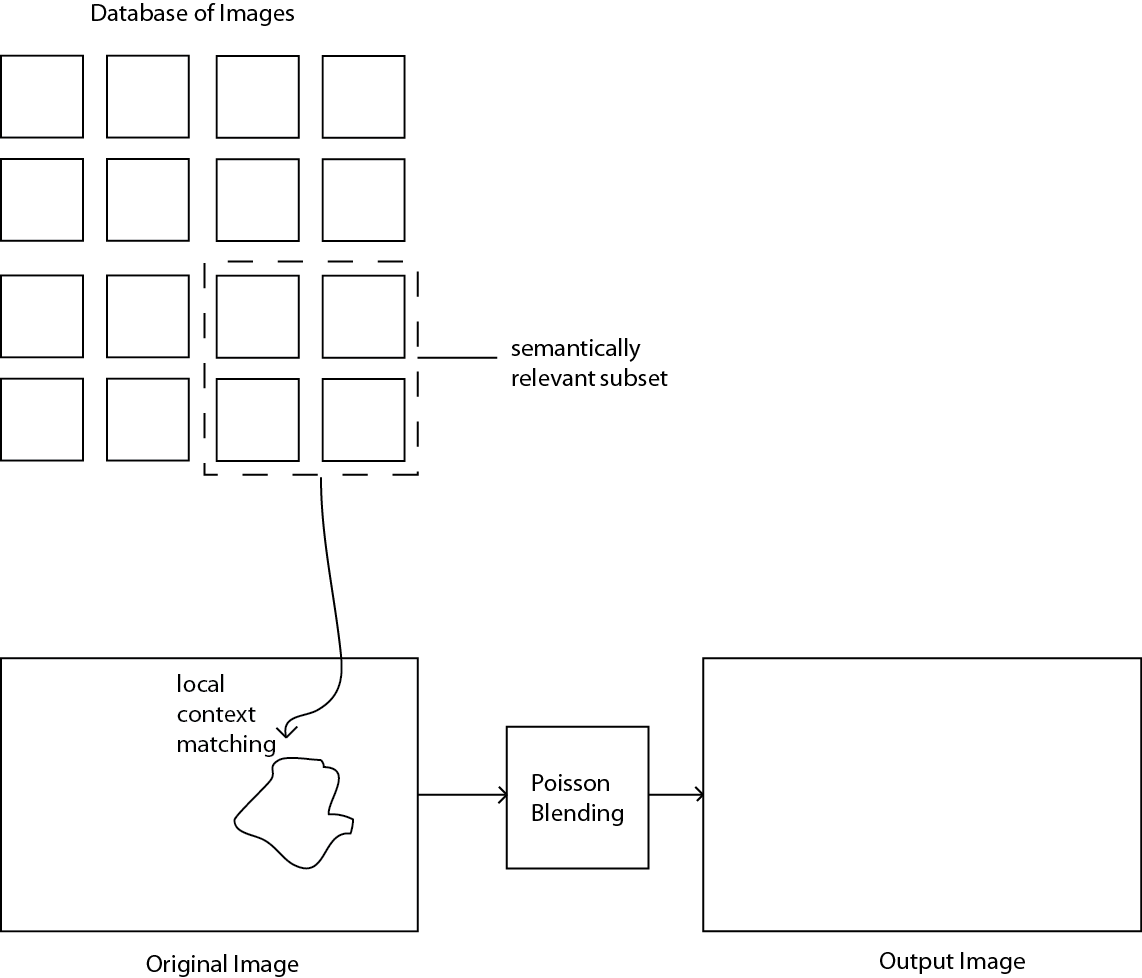
\includegraphics[scale=.5]{projectOverview.png}
\caption{Overview of scene completion.}
\label{scene}
\end{center}
\end{figure}

We also consider the problem of image resizing. One may wish to change the aspect ratio of an image without stretching or compressing the content of the image. We propose a new method of dynamic resizing based on the method of seam carving presented by Avidan and Shamir \cite{Avidan:2007} that takes advantage of Hays and Effros' work on scene completion. We carve a seam and then insert an image mask along that seam. This allows us to essentially cut the image along the seam and pull it apart. The scene completion algorithm then fills in the empty area around the seam with semantically relevant content as shown in Figure \ref{resize}. 

\begin{figure}[htbp]
\begin{center}
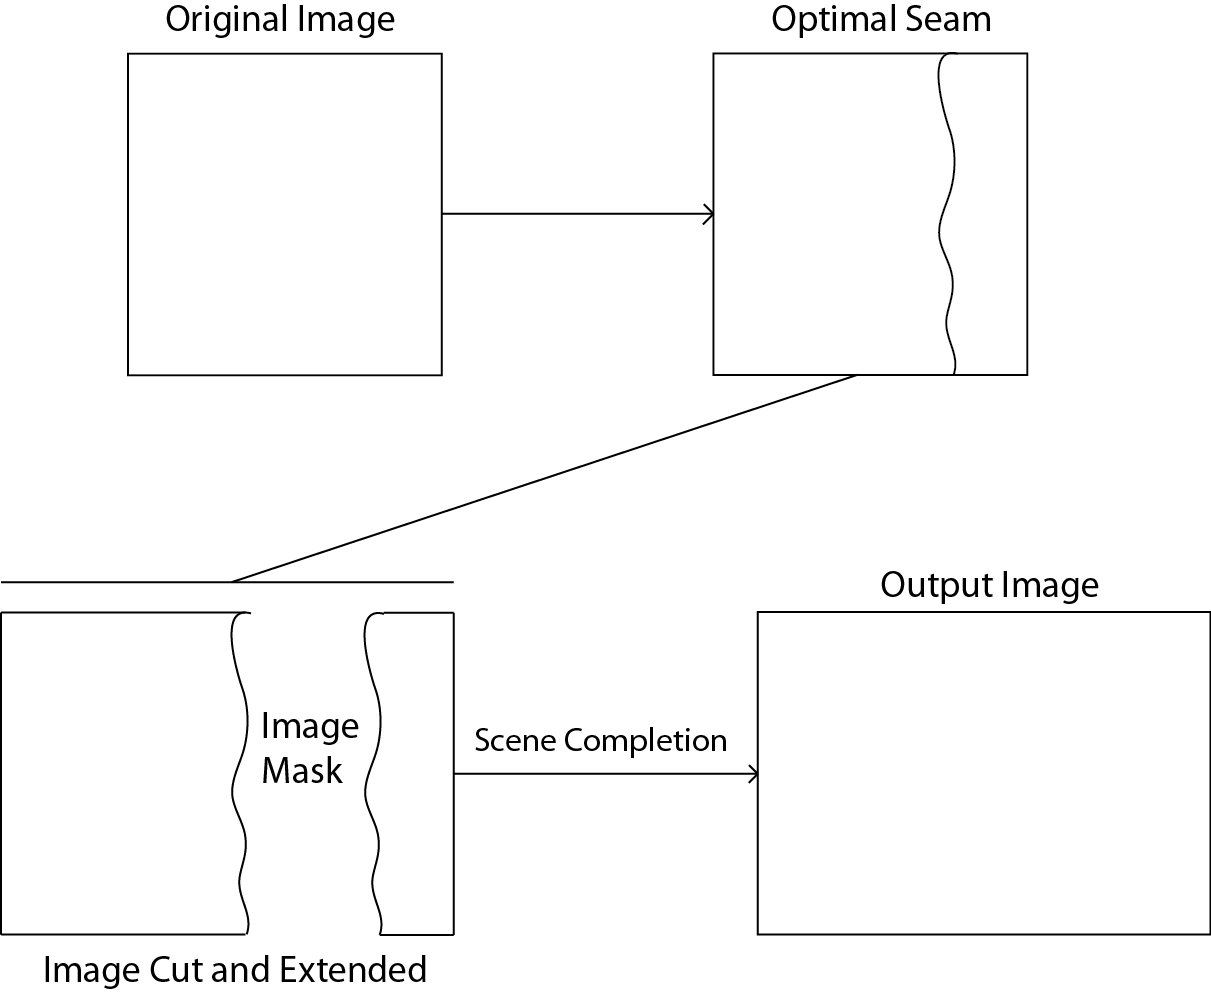
\includegraphics[scale=.5]{seamOverview.png}
\caption{Proposed resizing algorithm.}
\label{resize}
\end{center}
\end{figure}

\section{Overview} 
\subsection{Previous Work}
This paper is based largely on the work done by Hays and Efros \cite{Hays:2007} and
Avidan and Ahamir \cite{Avidan:2007}. There have been many papers published on the
topic of scene completion, but Hays and Efros are the first to propose a method that leverages
a large database of images downloaded from internet sources. 

The two basic strategies that have been explored in scene completion differ in the question that
they aim to answer. The first asks, ``what should have been there?'', while the second asks, ``what 
could have been there?'' \cite{Hays:2007}. Research in the first method tends to rely on multiple images of the input scene. Methods in the second camp tend to extend textures that already exist in the input image, such as the PatchMatch algorithm that is used as the basis for Content-Aware Fill in
Adobe Photoshop \cite{Barnes:2009}. The advantage of the method proposed by Hays and Efros is that is does not rely on either of these techniques. 

The image resizing algorithm proposed by Avidan and Ahamir has attracted a lot of attention due
to its simplicity and effectiveness. We use this paper as inspiration and take advantage of the seam carving algorithm that they proposed, but do not borrow their technique for resizing. Our resizing technique, to the best of our knowledge, is the first image resizing technique based on a scene
completion algorithm.

\subsection{Our Method}

We have implemented the method of scene completion proposed by Hays and Efros \cite{Hays:2007}. This algorithm allows a user to identify a certain area of an image to automatically be filled with new content. We also propose a novel use of this scene completion method in image resizing. This allows us to perform dynamic, content-aware image resizing based upon the seam carving method proposed by Avidan and Ahamir \cite{Avidan:2007}.

\section{Technical}

\subsection{Technical Summary}
Technical part: Summary of the technical solution 

\subsection{Technical Details}

We break this section up into two subsections, one for the scene completion algorithm, and one
for the seam carving algorithm. These sections contain the technical specifics necessary to implement 
the algorithms.

\subsubsection{Scene Completion Algorithm}

The scene completion algorithm can be broken down into four parts once the database of images has been created. The first part is to identify a subset of the database that is similar to the input image (semantic matching). The next part is to take each of these images and to find the best scale and translation for them to fill in the removed area (local context matching). After that, the most natural looking edge needs to be selected from the context area (graph-cut). Finally the last step is to perform a Poisson blend to make the final image look natural.

\paragraph{\sc Semantic Matching} 

Because the database of images is so large, it must be cut down to a relatively small subset of images before the local context matching can occur. If this were not the case, the algorithm would be computationally unfeasible (local context matching is the most expensive part of the process). 

In order to find images in the database that are most likely to yield a good local match, we try to find images in the database that are most semantically similar to the original image. We take advantage of prior work by Torralba and Oliva to define semantic similarity \cite{Torralba:2006}. We measure semantic similarity of two images by comparing taking the SSD of the gist descriptors of each image. In accordance with findings in previous work, we use gist descriptors with 6 oriented edge responses at 5 scales aggregated to a
4x4 spatial resolution \cite{Hays:2007}. We use the $n$ images that are semantically closest to the original
for the local context matching step. 

\paragraph{\sc Local Context Matching}


We follow the context matching method proposed by Hays and Efros.\cite{Hays:2007} Given the target image, a semantically similar source image, and a user-defined selection, we must find an optimal translation and scale of the source. The optimal fit is found by finding the minimum sum of squared distances error. The error is computed by finding the SSD of pixel values and the SSD of a 5x5 pixel median filter on both images which acts to match similar textures. The algorithm iterates over all possible translations and a range of scales to find the optimal fit. The exhaustive nature of this method is computationally taxing; it is only feasible to run the method on a small set of images.


\paragraph{\sc Graph Cut}

Following the method of Hayes and Effros \cite{Hays:2007} we allow for dynamic expansion of the border around the area of the image which is to be replaced. That is, we allow the area to expand (up to 80 pixels in any direction) but not contract. The reasoning behind this is that it will allow for a more natural integration of the match image into the original image. Contraction of the area is not allowed because this could possibly cause specific objects that the user is trying to delete to remain in the image. 


The problem then is to identify the border which will make the match look the most natural. This formulation can be reduced to a graph cut problem. We take each pixel in the context region (the 80 pixel buffer around the original selection) and treat it as a vertex on a graph. Then, we assign weights to each of the edges. The weights are based on the following formula

\begin{displaymath}
	w_{i,j} = \left\{ 
		\begin{array}{lr}
			\triangledown diff(i,j) + (k \cdot Dist(i,hole))^3 &  i,j \in context \\
			0 &  otherwise
		\end{array}
	\right.
\end{displaymath}

where $i,j$ are adjacent pixels, $\triangledown diff(i,j)$ is the magnitude of the gradient of the SSD between the images, and $k \approx .002$ is an empirical constant presented by Wilczkowiak, et. al. \cite{Gabriel:2005}. This takes into account the visual cost of having these two pixels be from different images and also adds a penalty for pixels as they are farther away from the hole area. We use the algorithm proposed by Karger \cite{Karger:1992} to find the minimum graph cut, and hence the label for each pixel in the context area.

\paragraph{\sc Poisson Blending}



A method is needed to combine the target image and the source image given by the local context matching. Simply pasting the images together may result in a jarring transition with mismatching color values. Poisson blending alleviates this by operating on the source image gradient; a solution is found which minimizes the changes to the gradient while obeying boundary conditions which match the pixel values in the source on the edge of the context to the target image. The resulting image features a smooth transition with matching color values while preserving the contents of the source image.


We use poisson blending as described in P$\acute{e}$rez et. al. \cite{Perez:2003} We define $f$ to be the unknown portion of the target image in the context $\Omega$. The known portion of the image is defined as $f^\ast$ and the gradient of the source image is defined as $v$. To successfully blend the images we must solve the following minimization problem:

$$ 
\min_f \iint_\Omega|\nabla f-v|^{2} \;\mathrm{with}\; f|_{\partial\Omega} = f^{\ast}|_{\partial\Omega} 
$$

$\nabla$ is the gradient operator and $\partial\Omega$ is the boundary of the context area. The above equation's solution is the unique solution to the following Poisson equation:

$$
\Delta f=\mathrm{div} v\;\mathrm{ over }\;\Omega\;\mathrm{  with}\;  f|_{\partial\Omega} = f^{\ast}|_{\partial\Omega}
$$

$\Delta f = \frac{\partial^{2} f}{\partial^{2}x^2}+\frac{\partial^{2}f}{\partial^{2}x^2}$ is the Laplacian operator and $\mathrm{div} v = \frac{\partial u}{\partial x}+\frac{\partial v}{\partial y}$ is the divergence of the gradient $v=(u,v)$.


\subsubsection{Dynamic Resizing}

We use the seam finding algorithm proposed by Avidan and Shamir \cite{Avidan:2007} as the basis of our dynamic resizing algorithm. 

\begin{figure}[htbp]
\begin{center}
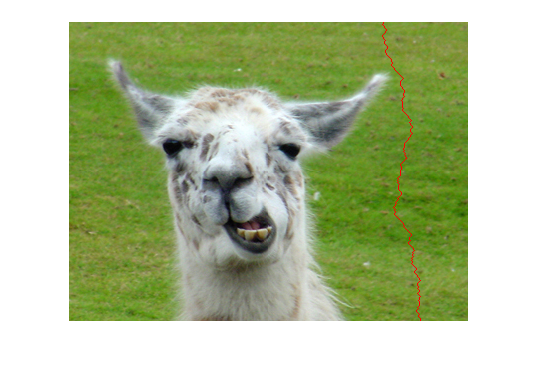
\includegraphics[scale=.38]{seam.png}
\caption{An optimal seam displayed on an image of a llama.}
\label{llamaSeam}
\end{center}
\end{figure}


We find the optimal seam  

$$ 
s^* = \min_s E(s) = \min_s \sum^n_{i=1} e(\mathbf{I}(s_i))
$$

where $\mathbf{I}(s_i)$ is the intensity of the image at $s_i$ and $e$ is an energy function defined as

$$
e(\mathbf{I}) + |\frac{\delta}{\delta x} \mathbf{I} | + | \frac{\delta}{\delta y} \mathbf{I} |
$$ 

The optimal seam can be computed efficiently by using dynamic programming. To do this, the cumulative energy function $M$ must be found for each pixel on the last row or column of the image (depending on
whether the seam is vertical or horizontal). $M$ is defined for a vertical seam as

$$
M(i,j) = e(i,j) + \min(M(i-1,j-1), M(i-1, j), M(i-1, j+1))
$$

The definition of $M$ for horizontal seams is symmetric. Once this seam is computed, a user defined amount
of empty pixels are inserted into the images along the seam, as seen in Figure \ref{llamaCut}. These empty pixels are used as an image mask, and the image is then passed as input to the scene completion algorithm.

\begin{figure}[htbp]
\begin{center}
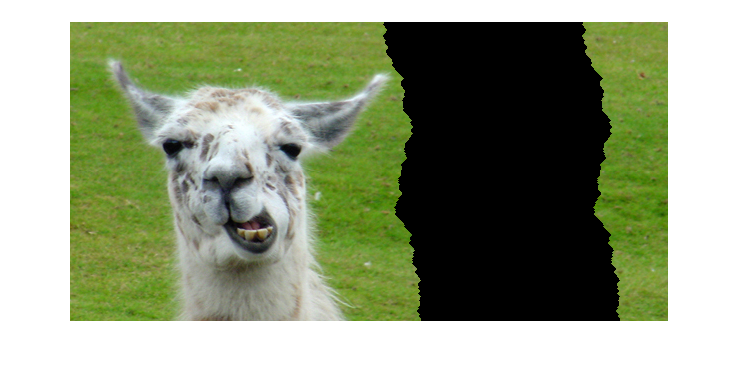
\includegraphics[scale=.4]{broken.png}
\caption{An image cut along the optimal vertical seam and extended horizontally 200 pixels.}
\label{llamaCut}
\end{center}
\end{figure}


\section{Experiments}

The best available metric for determining the success of this algorithm is to present the output images (the completed scenes) and let humans determine if they appear natural or not. Unfortunately there is no better way to quantize this than to distribute the output images to be judged by impartial test subjects \cite{Hays:2007}, but the time frame of this project did not allow for such experiments. Here we show output images, both good and bad, and provide commentary on them and how they display a strength or weakness of the algorithmm. Overall we found the algorithm to be relatively ineffective \emph{unless} there was a near exact match in the image database.

\subsection{Preliminary Results ($\approx14000$ images)}

We began testing the scene completion algorithm when we had built up a database of approximately fourteen thousand images. This is considerably less than the two million images used in \cite{Hays:2007}, but we wanted to test how much of a difference having more images made.

\begin{figure}[h]
\begin{center}$
\begin{array}{ccc}
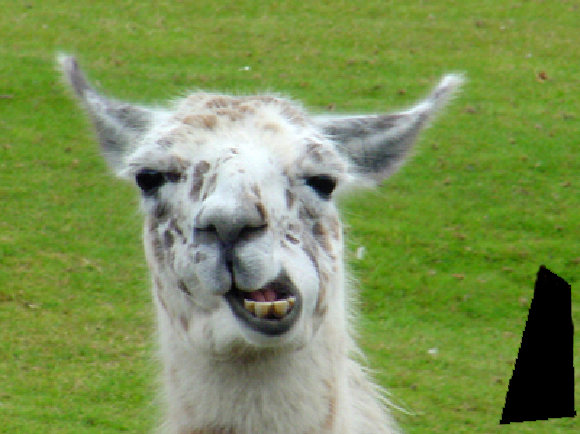
\includegraphics[width=1.8in]{mask.png} &
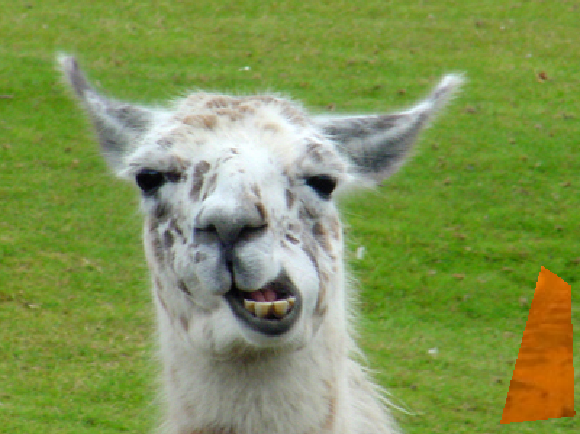
\includegraphics[width=1.8in]{filled.png} &
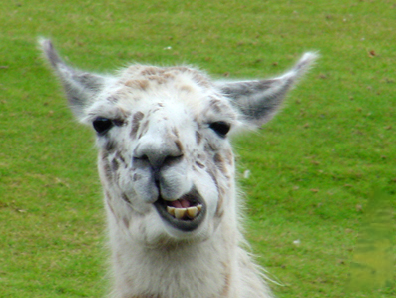
\includegraphics[width=1.8in]{blended.png} 
\end{array}$
\end{center}
\caption{Successful scene completion using only fourteen thousand images.}
\label{llamaMatch}
\end{figure}

\begin{figure}[h]
\begin{center}$
\begin{array}{cc}
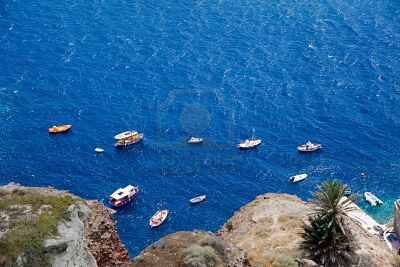
\includegraphics[width=2.3in]{sailboat.jpg} &
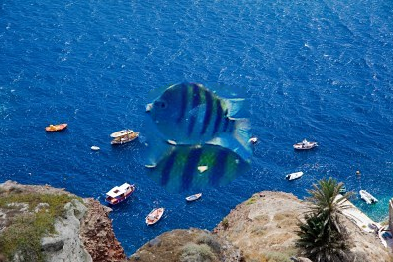
\includegraphics[width=2.3in]{fish2.png}
\end{array}$
\end{center}
\caption{Semantically incorrect completion.}
\label{badMatch}
\end{figure}

With a database this size, there was seldom a close enough match image to provide satisfactory results. Occasionally we would get output images that were semantically incorrect yet still looked somewhat natural, as seen in Figure \ref{badMatch}. We had success doing scene completion when we removed areas of the area that we heterogeneous in content (such as a patch of an image that was all one texture, e.g. a patch of grass), as in Figure \ref{llamaMatch}.

\subsection{Further Results ($\approx100000$ images)} 

Expanding our database to over one-hundred thousand images increased the robustness of 
the scene completion algorithm. We were able to fill in more complex areas of an image, but
it was still not perfect. The computational cost of this algorithm made it difficult given the time constraints, so we were not able to build a database as large as that of Hays and Effros. We believe 
that these results show that we have produced a sound implementation of the algorithm that would
continue to perform better as more images were added to the database.

\begin{figure}[h]
\begin{center}$
\begin{array}{cc}
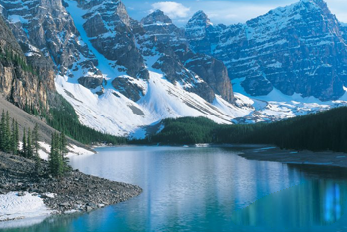
\includegraphics[scale=.3]{mountains100kInsert.png} &
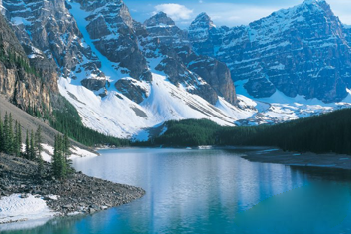
\includegraphics[scale=.3]{mountainsInsert2.png} \\
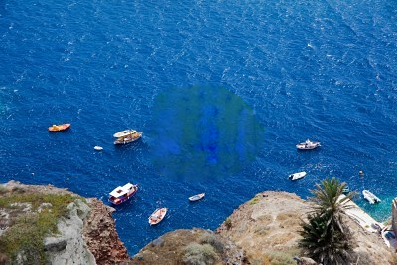
\includegraphics[scale=.3]{water100k.png} & 
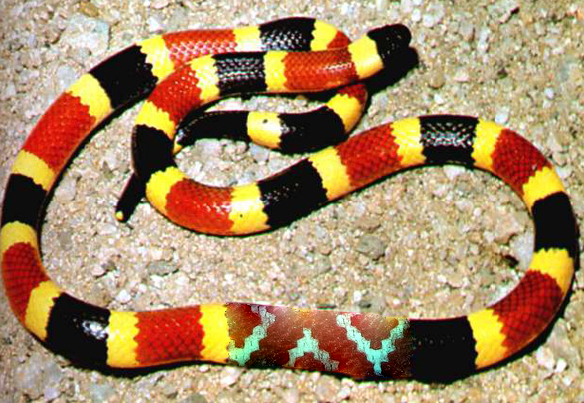
\includegraphics[scale=.2]{snake.png}
\end{array}$
\end{center}
\caption{Some completed scenes.}
\label{vertResize}
\end{figure}


\subsection{Dynamic Resizing}

Our results for dynamic image resizing using scene completion were unimpressive, but this must be due in part to the size of our database. The area of that needed to be filled in by the scene completion algorithm was particularly awkward if the user wanted to resize in both the horizontal and vertical directions. This made finding an accurate match image even more difficult. 


\begin{figure}[htbp]
\begin{center}$
\begin{array}{cc}
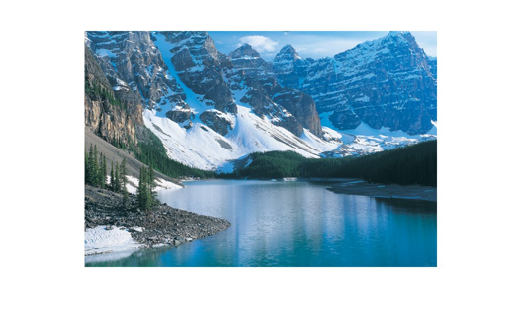
\includegraphics[scale=.3]{mountains.png} &
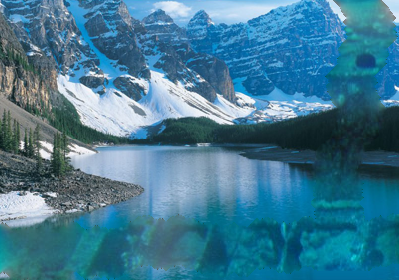
\includegraphics[scale=.3]{resize1.png}
\end{array}$
\caption{Vertical and horizontal expansion.}
\label{bothResize}
\end{center}
\end{figure}

Results of resizing in only one direction showed more promise, but the area to complete was so large that they were not perfect. We believe that a much larger image database is necessary to get natural looking results for our proposed resizing algorithm.

\begin{figure}[h]
\begin{center}$
\begin{array}{cc}
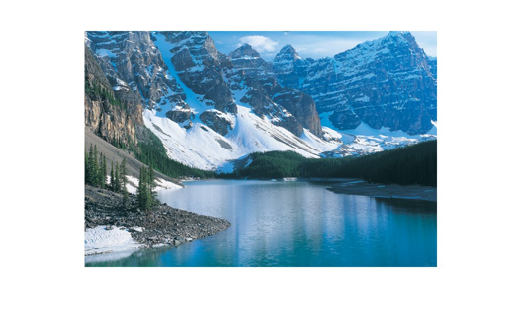
\includegraphics[scale=.3]{mountains.png} &
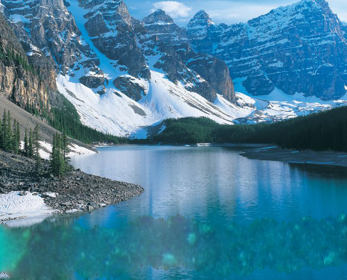
\includegraphics[scale=.3]{1resize.png} \\
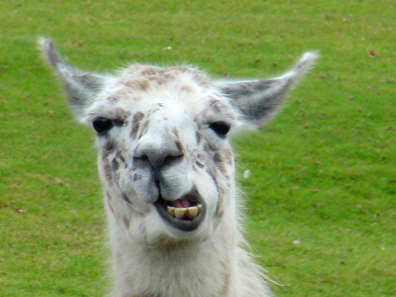
\includegraphics[scale=.3]{llama.png} &
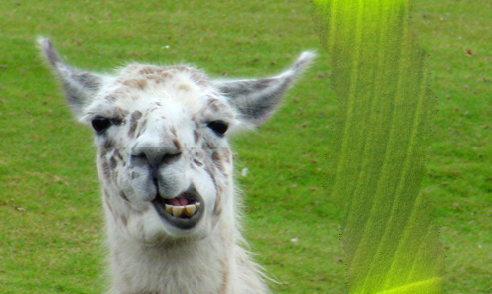
\includegraphics[scale=.3]{llamaResize.png}
\end{array}$
\end{center}
\caption{Single direction resizing results.}
\label{vertResize}
\end{figure}


\section{Conclusion}

\subsection{Current Results}

Our results confirm that it is possible to leverage a large database of images in order to perform
scene completion. The drawback of this method is that it is computationally expensive and requires
a near exact match image to be found in the database. This method also requires the large 
upfront cost of constructing the database. Because of time constraints our database was not as
large as that in \cite{Hays:2007} and hence our implementation was not as robust. That being said,
we still saw some promising results and were able to see some natural looking output images. We 
believe that our implementation of the algorithm was sound and would have continued to increase in
performance as we added more images to the database.

Our proposed method of image resizing using seam completion did not produce many natural looking results. It did however point out one of the weaknesses of this method of seam completion: as the 
area of completion grows larger, the Poisson blending becomes increasingly less effective.

\subsection{Future Work}

As it stands, this algorithm is not suitable for widespread use because of the extensive runtime and requirement of a large local database. A future project may include setting up a web service that would allow a user to upload an image and mask, and then return a semantically close set of images. This would allow researchers to implement the rest of the scene completion without requiring them to compile a huge amount of images.

\bibliographystyle{plain}
\bibliography{bibliography}

\end{document}  